\documentclass[11pt]{article}

\usepackage[T2A]{fontenc}
\usepackage[utf8]{inputenc}
\usepackage[russian]{babel}

\usepackage{indentfirst}
\usepackage{geometry}

\usepackage{amsmath, amssymb, amsfonts, amsthm, amscd}
\usepackage{mathrsfs}

\usepackage{caption}
\usepackage{graphicx}
\usepackage[all]{xy}

\geometry{a4paper}
\sloppy


\theoremstyle{plain}
\newtheorem{lemma}{Лемма}
\newtheorem{statement}{Утверждение}
\newtheorem{theorem}{Теорема}
\theoremstyle{definition}
\newtheorem{definition}{Определение}
\newtheorem{corollary}{Следствие}
\theoremstyle{remark}
\newtheorem*{remark}{Замечание}

\renewcommand{\le}{\leqslant}
\renewcommand{\ge}{\geqslant}
\renewcommand{\phi}{\varphi}
\renewcommand{\epsilon}{\varepsilon}
\renewcommand{\kappa}{\varkappa}

\newcommand{\comdots}{,\!..}
\newcommand{\sub}[1]{\lfloor #1 \rfloor}

\DeclareMathOperator*{\Hom}{Hom}
\DeclareMathOperator*{\Tor}{Tor}
\DeclareMathOperator*{\Obj}{Obj}
\DeclareMathOperator*{\Arr}{Arr}
\DeclareMathOperator*{\fund}{fund}
\DeclareMathOperator*{\codom}{codom}
\DeclareMathOperator*{\id}{id}
\DeclareMathOperator*{\subdim}{\lfloor \dim \rfloor}

\renewcommand{\thesubsubsection}{\roman{subsubsection}.}

\begin{document}

\author{А.~A.~Владимиров}
\title{Характер группоида}
\date{16.06.2022}
\maketitle

\section*{Задача}

    Дан функтор $\kappa = (\kappa_1, \kappa_2): \mathbf{Cat}(\Gamma) \to 
    \mathbf{Vec}$.\\
    Найти $\kappa_2 : (f: \Gamma_1 \to \Gamma_2) \mapsto 
    (A_f: \kappa_1(\Gamma_1) \to \kappa_1(\Gamma_2))$, если известно, что 
    $\kappa_1 : \Gamma \mapsto V$, где $V$ -- пространство характеров, т.е. 
    $V = \{\chi: \Hom \Gamma \to \mathbb{C}: \chi(\psi \circ \phi) = 
    \chi(\psi) + \chi(\phi)\}$.

    Таким образом задача сводится к нахождению линейного оператора $A_f$ на 
    коммутативной диаграмме 

    \begin{figure}[h]
        \centering
        \[\xymatrix{
            \Gamma_1 \ar[dd]^{\textstyle{f}} \ar[rr]^{\textstyle{\kappa}} & & V_1 \ar[dd]^{\textstyle{A_f}} \\
                                            & & \\
            \Gamma_2 \ar[rr]^{\textstyle{\kappa}}           & & V_2
        }\]
        \caption{постановка задачи}
        \label{cd_problem}
    \end{figure}

\section*{Решение}
\tableofcontents

\newpage    \subsection{Структура группоида}
            
    Перед тем, как ислледовать характеры, обсудим сперва саму структуру группоида
    \footnote{здесь и далее под группоидами подразумеваются связные группоиды}.

    \begin{definition}\cite{MacLane}
        \emph{Группоидом} назывется категория, любая стрелка которой обратима.
    \end{definition}

    \begin{figure}[h]
        \centering
        \[\xymatrix{
            b \ar@(u,l)[]_{\hom(b,b)} \ar[ddrr]^{\hom(b,c)}                     & &                             \\
                                                                                & &                             \\
            a \ar@(l,d)[]_{\hom(a,a)} \ar[uu]^{\hom(a,b)} \ar[rr]_{\hom(a,c)}   & & c \ar@(r,d)[]^{\hom(c,c)}
        }\]
        \caption{группоид}
        \label{cd_groupoid}
    \end{figure}

    Попытаемся найти в группоиде ``что-то вроде базиса''. В некотором 
    группоиде $\Gamma$ выберем произвольную вершину $a$ и рассмотрим её группу 
    петель $G$ и \emph{веер стрелок} $(e, f, g,\ldots)$.

    \begin{definition}
        \emph{Веером стрелок} вершины $a$ группоида $\Gamma$ назовем 
        множество стрелок 
        $V = \{e = \id_a : a \to a,\: f: a \to b,\: g: a \to b,\: \ldots\}$, 
        исходящих из вершины $a$ по одной в каждую из вершин группоида, причем 
        $e : a \to a$ есть тождественная стрелка.
    \end{definition}

    \begin{figure}[h]
        \centering
        \[\xymatrix{
            b                                                                           & &     \\
                                                                                        & &     \\
            a \ar@(l,d)[]_{\textstyle e} \ar[uu]^{\textstyle f} \ar[rr]_{\textstyle g}  & & c
        }\]
        \caption{веер}
        \label{cd_groupnfan}
    \end{figure}

    Возникает вопрос: как соотносятся с выделенным ``базисом'' остальные 
    стрелки группоида? Ответ на него дает следующая простая лемма.

    \begin{lemma}\label{lm_1} Для любой стрелки $v : b \to c$ группоида 
        $\Gamma$ существуют, и притом единственные $f,g \in V$ и $h \in G$, 
        такие что
            \begin{equation}\label{arr_represent}
                v = ghf^{-1}.
            \end{equation}
    \end{lemma}
    \begin{proof}
        Действительно, поскольку $v : b \to c$, и $h : a \to a$, стрелки $g$ и 
        $f$ обязаны действовать из $a$ в $c$, и из $a$ в $b$ соответственно, а 
        таковые имеются в $V$ в единственном экземпляре.
        
        Раз теперь известны $v$, $g$ и $f$, существование и единственность 
        стрелки $h \in G$ следует напрямую алгебраически из выражения 
        \eqref{arr_represent}, а именно $h = g^{-1}vf$.
    \end{proof}
    
    Иными словами, мы построили биекцию 
    \begin{equation}\label{iota}
        \iota : \Arr(\Gamma) \to V \times G \times V
    \end{equation}
     --- между стрелками и множеством троек вида $ghf^{-1}$.

    Располагая таким построением, мы опустим кавычки говоря о $(G,V)$ как о 
    \emph{базисе} группоида $\Gamma$, а под \emph{разложением} по этому базису 
    стрелки или множества стрелок с математической точки зрения будем 
    подразумевать образ соответствующего множества при отображении $\iota$.

    Перебирая и фиксируя различные пары $(g,f)$ можно получить разложение 
    группоида по базису $(G, V)$, о чем и говорит
    
    \begin{corollary}\label{cor_repres} (о представлении $\hom$-множеств)
        \begin{itemize}
            \item[a.] $\hom(b,c) = gGf^{-1}$
            \item[b.] $\hom(a,b) = fGe^{-1} = fG$,
            \item[c.] $\hom(b,a) = eGf^{-1} = Gf^{-1}$,
            \item[d.] $\hom(b,b) = fGf^{-1}$, \footnote{Это классическое 
            утверждение об изоморфности всех групп петель в группоиде (которое 
            и позволяет ввести такой объект как фундаментальная группа)}
            \item[e.] $\hom(a,a) = eGe^{-1} = G$,
        \end{itemize}
        где $f : a \to b$, $g : a \to c$, $G = \hom(a,a)$.
    \end{corollary}

    Полезно также отедельно выделить частный случай.

    \begin{definition}
        \emph{Простым группоидом} назовем группоид, фундаментальная группа 
        которого тривиальна.
    \end{definition}

    Для которого, ввиду $G = \{\id_a$\} следствие \ref{cor_repres} принимает вид:

    \begin{corollary}\label{cor_simple_grp}
        В простом группоиде любая стрелка $v : b \to c$, раскладывается в 
        базисе $V$ как
        \[v = gf^{-1},\]
        где $f : a \to b$, $g : a \to c$.
    \end{corollary}
    
    \begin{figure}[h]
        \centering
        \[\xymatrix{
            b \ar@(u,l)[]_{\textstyle fGf^{-1}} \ar[ddrr]^{\textstyle gGf^{-1}}             & &                             \\
                                                                                            & &                             \\
            a \ar@(l,d)[]_{\textstyle G} \ar[uu]^{\textstyle fG} \ar[rr]_{\textstyle gG}    & & c \ar@(r,d)[]^{\textstyle gGg^{-1}}
        }\]
        \caption{фактор-группоид}
        \label{cd_groupoid_repres}
    \end{figure}

    Вернемся к группоиду $\Gamma$ и перерисуем диаграмму \ref{cd_groupoid} с 
    учетом следствия \ref{cor_repres} (рис.~\ref{cd_groupoid_repres}). 
    Диаграмма \ref{cd_groupoid_repres} напоминает некую ``факторизацию'', и 
    действительно, если под стрелками на диаграмме понимать не $\hom$-множества,
    а просто стрелки, то мы получим диаграмму \emph{фактор-группоида} 
    $\Gamma/\Phi_\Gamma$\footnote{Пользуясь стандартным 
    определением факторизации категории\cite{MacLane}, естественным
    образом, подобно тому как это делается в обыкновенных группах, можно ввести 
    факторизацию группоида по любой нормальной подгруппе фундаментальной 
    группы, в том числе и по ней самой.} по фундаментальной группе $\Phi_\Gamma$, 
    где названия стрелок соответствуют прообразам 
    факторизации. Мы не будем здесь строго вводить понятие фактор-группоида, 
    ибо в нашем случае он предствляет из себя всего-навсего \emph{простой 
    группоид} с тем же набором объектов что и исходный.

    При виде диаграммы \ref{cd_groupoid_repres} кажется само собой разумееющимся
    \begin{statement}[о разложении группоида]\label{st_groupoid_decomp}
        \begin{equation}
            \Gamma \simeq \textstyle{\Gamma / \Phi_\Gamma \times \Phi_\Gamma}.
        \end{equation}
    \end{statement}

    Перед доказательством утверждения \ref{st_groupoid_decomp} напомним тот 
    факт, что \emph{группа является категорией --- частным случаем группоида с одним 
    объектом}, и 
    \begin{definition}\cite{MacLane}
        \emph{Произведением} двух данных категорий $B$ и $C$, называется 
        категория $B \times C$, объекты которой~--- пары $(b,c)$ объектов $b$ из 
        $B$ и $c$ из $C$; стрелки $(b,c) \to (b',c')$~--- пары $(f,g)$ стрелок 
        $f : b \to b'$ и $g : c \to c'$, a композиция двух таких стрелок
        \[(b,c) \stackrel{(f,g)}{\longrightarrow} (b',c') \stackrel{(f',g')}{\longrightarrow} (b'',c'')\]
        определяется в терминах композиции в категориях $B$ и $C$ по формуле
        \[(f',g') \circ (f,g) = (f' \circ f, g' \circ g).\]
    \end{definition}

    \begin{proof}
    
        Построим явно изоморфизм~--- функтор $i : \Gamma \to 
        \Gamma / \Phi_\Gamma \times \Phi_\Gamma$.

        Для этого выделим некоторый базис $(G = \hom(a,a), V\text{~--- веер } a)$ 
        группоида $\Gamma$, и для удобства отождествим $\Phi_\Gamma$ с $G$, а 
        веер вершины $a$ в $\Gamma / \Phi_\Gamma$ с $V$.

        Тогда $i$ зададим следующим образом:
        \begin{itemize}
            \item [на объектах:] $i : d \mapsto (d,\theta)$;
            \item [на стрелках:] $i : v \mapsto (gf^{-1},h)$, где 
            $(g,h,f^{-1}) = \iota(v)$.
        \end{itemize}

        Биективность и функторность $i$ очевидна вследствие определения 
        биекции $\iota$, леммы \ref{lm_1} и ее следствий. Впрочем, в этом также 
        можно наглядно убедится взглянув на схему, 
        изображенную на рис.~\ref{cd_groupoid_iso}.

        \begin{figure}[h]
            \centering
            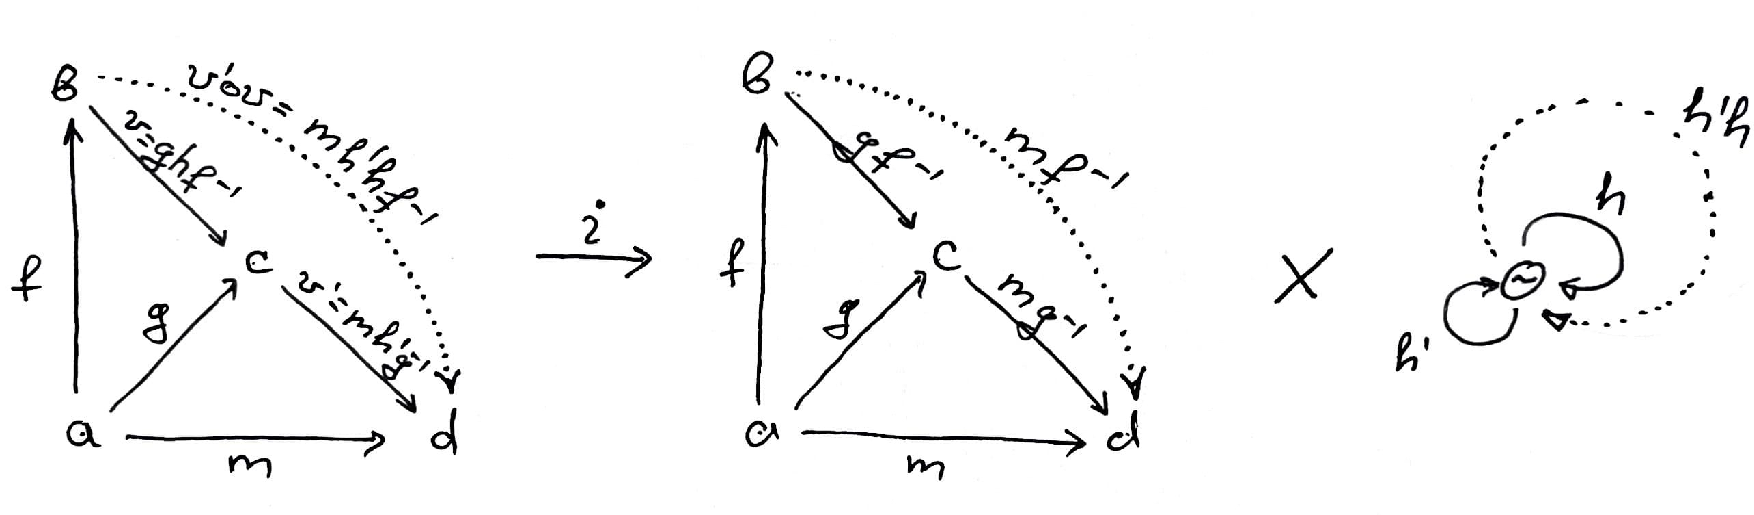
\includegraphics[width=\textwidth]{pictures/cd_grp_iso.pdf}
            \caption{изоморфизм}
            \label{cd_groupoid_iso}
        \end{figure}
    \end{proof}

        Теперь мы готовы перейти к обсуждению характера.

\newpage    \subsection{Пространство характеров}
            \subsubsection{Группоид}
    Нам потребуется следующая очевидная

    \begin{lemma}\label{lm_char_decomp}
        Для любых двух группоидов $\Gamma_1$ и $\Gamma_2$ справедливо
        \[X(\Gamma_1 \times \Gamma_2) \simeq X(\Gamma_1) \oplus X(\Gamma_2).\]
    \end{lemma}
    \begin{proof}
        В самом деле, для любого $\chi : \Gamma_1 
        \times \Gamma_2 \to \mathbb{C}$, существуют единственные
        $\chi_1 : \Gamma_1 \to \mathbb{C}$, $\chi_2 : \Gamma_2 \to \mathbb{C}$ 
        такие, что диаграмма (рис.~\ref{cd_char_sum}) коммутативна.

        \begin{figure}[h]
            \centering
            \[\xymatrix{
                \Gamma_1 \times \Gamma_2 \ar[rr]^{\textstyle \chi_b \times \chi_c} \ar[dd]_{\textstyle \chi_a}  & & \mathbb{C} \times \mathbb{C} \ar[lldd]^{\textstyle +}\\
                                                                                                                & &                                                      \\
                \mathbb{C}                                                                                      & &
            }\]
            \caption{}
            \label{cd_char_sum}
        \end{figure}
    \end{proof}

    Доказанная лемма вместе с утверждением \ref{st_groupoid_decomp} 
    дают важное
    \begin{statement}[о разложении характера группоида]\label{st_char_grpd_decomp}
        \[X(\Gamma) \simeq X(\Gamma/\Phi_\Gamma) \oplus X(\Phi_\Gamma).\]
    \end{statement}

    Которое позволяет нам вместо рассмотрения характера на группоиде целиком,
    отдельно изучить характеры \emph{простого группоида} ($\Gamma/\Phi_\Gamma$) и
    группы ($\Phi_\Gamma$).

    Первый случай достаточно тривиален. Действительно, как уже было показано 
    (следствие \ref{cor_simple_grp}), все стрелки простого 
    группоида можно однозначно разложить\\ $v = gf^{-1}$ по некоторому вееру $V$,
    что ввиду свойств характера дает его выражение через значения на базисе 
    $\chi(v) = \chi(g) - \chi(f)$.

    Отсюда ясно, что характер простого группоида 
    однозначно определен $n-1$\footnote{значение на тождественной стрелке 
    автоматически задано нулем} числом~--- его значениями на стрелках некоторого 
    веера. Иначе говоря справедливо

    \begin{statement}\label{st_smp_grp_char} Для простого группоида $\Gamma$
        \[X(\Gamma) \simeq \mathbb{C}^{n-1},\]
        где $n$~--- число объектов $\Gamma$.
    \end{statement}

    Случай группы мы обудим в следующих параграфах.

            \subsubsection{Простой группоид}
    Напомним некоторые свойства характера:
    \begin{itemize}
        \item[a.] $\chi(fg) = \chi(f) + \chi(g)$
        \item[b.] $\chi(f^{-1}) = - \chi(f)$
        \item[c.] $\chi(\id) = 0$
    \end{itemize} 
    
    Как было показано (следствие \ref{cor_simple_grp}) все стрелки простого 
    группоида можно однозначно разложить $v = gf^{-1}$ по некоторому вееру $V$,
    а из свойств a.--c.: $\chi(v) = \chi(g) - \chi(f)$.

    Отсюда ясно, что характер простого группоида 
    однозначно определен $n-1$\footnote{значение на тождественной стрелке 
    автоматически задано нулем} числом~--- его значениями на стрелках некоторого 
    веера. Иначе говоря справедливо

    \begin{statement} Для простого группоида $\Gamma$
        \[X(\Gamma) \simeq \mathbb{C}^{n-1},\]
        где $n$~--- число объектов $\Gamma$.
    \end{statement}

    Разобравшись с первой состовляющей характера группоида (характером 
    простого группоида), перейдем ко второй --- характеру группы.
            \subsubsection{Группа}
    Рассмотрим некоторую группу $G$, ее фактор-группу $G/G'$ по коммутанту 
    $G'$ и следующую диаграмму

    \begin{figure}[h]
        \centering
        \[\xymatrix{
            G \ar[rr]^{\textstyle{\tau}} \ar[rrdd]_{\textstyle{\chi}} & & G/G'\ar[dd]^{\textstyle{\chi_{ab}}} \\
            & & \\
            & & \mathbb{C}
        }\]
        \caption{}
        \label{cd_ab}
    \end{figure}

    Здесь $\tau: g \mapsto gG'$ --- канонический гомоморфизм; $\chi$, 
    $\chi_{ab}$ --- характеры групп $G$ и $G/G'$ соответственно.

    Оказывается, что 

    \begin{lemma}\label{lm_const} Для любых $f, g \in G$, таких что $f = g \mod G'$:
        \[\chi(f) = \chi(g).\]
    \end{lemma}

    \begin{proof} Действительно, в условиях леммы существует $h \in G'$, 
        такой что $f = gh$, но по определению коммутанта существуют такие 
        $a$ и $b \in G'$, что \\$h = aba^{-1}b^{-1}$, откуда $f = gaba^{-1}b^{-1}$, и 
        \[\chi(f) = \chi(gaba^{-1}b^{-1}) 
        = \chi(g) + \chi(a) + \chi(b) - \chi(a) - \chi(b) = \chi(g).\]
    \end{proof}

    Иными словами доказано, что факторизация 
    группы по коммутанту $G'$ разбивает ее на области постоянства
    характера (рис. \ref{img_chi_factor}). А значит вместо 
    рассмотрения характера $\chi$ на всей группе, достаточно пронаблюдать 
    лишь за его "<действием с точностью до $G'$">, т.е. за некоторым характером
    $\chi_{ab}$ на $G/G'$.

    \begin{figure}[h]
        \centering
        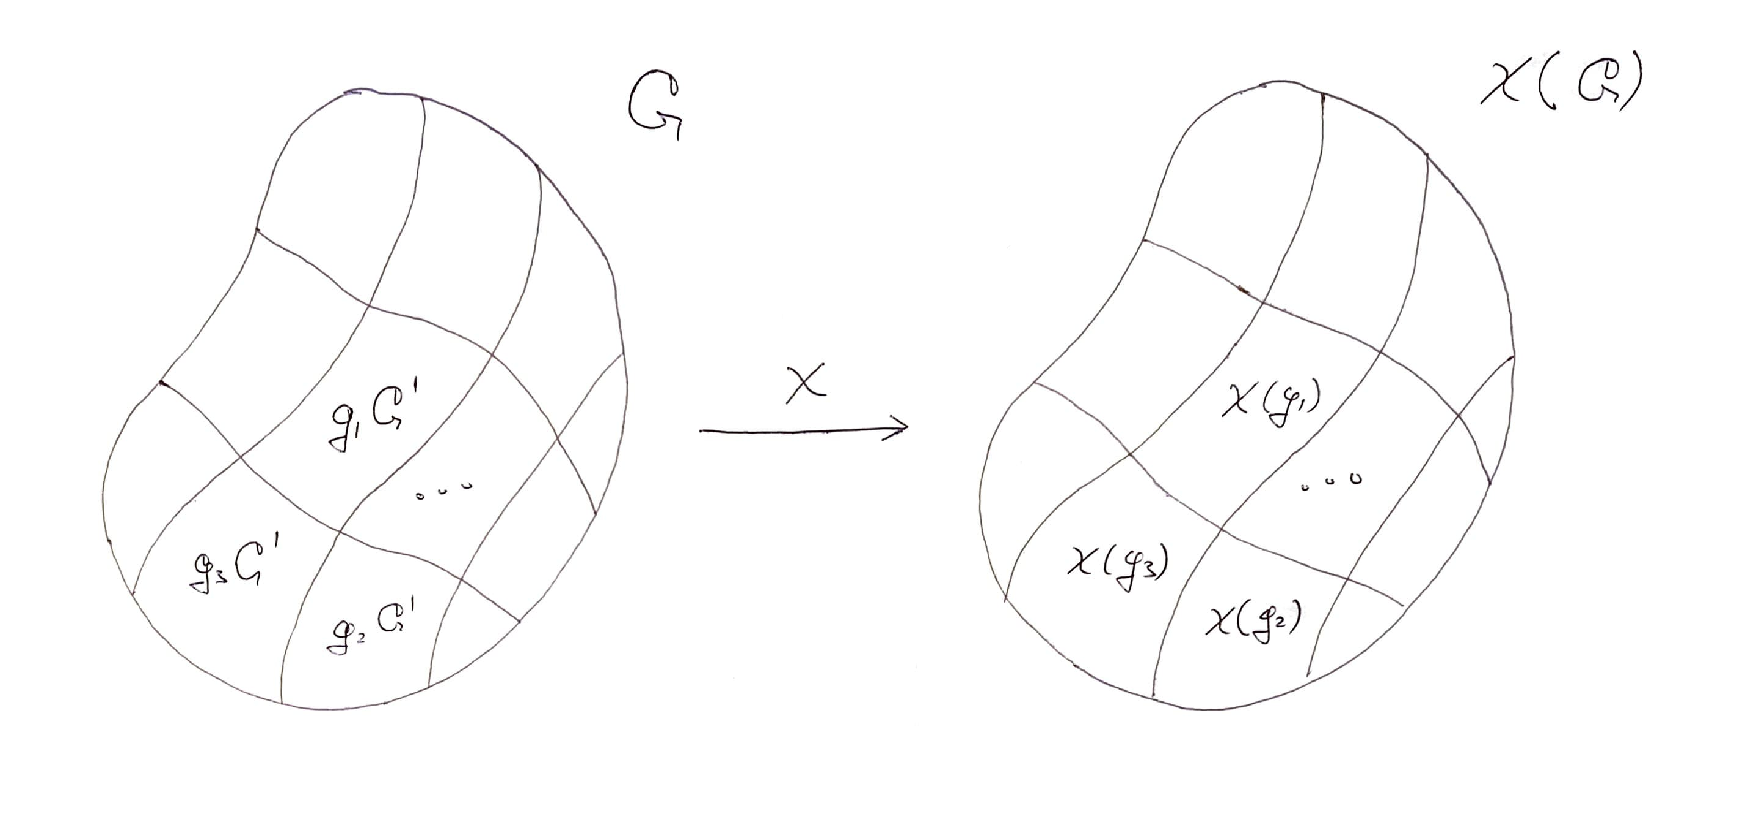
\includegraphics[width=\textwidth]{pictures/chips}
        \caption{}
        \label{img_chi_factor}
    \end{figure}

    Так, введем, очевидно инъективный, гомоморфизм 
    $t: X(G/G') \to X(G)$ пространств характеров:
    \begin{equation}
        t : \chi_{ab} \mapsto \chi_{ab} \circ \tau = \chi. 
    \end{equation}
    Его сюръективность вытекает напрямую из леммы \ref{lm_const}, ибо для 
    любого $\chi : G \to \mathbb{C}$ корректно задан $\chi_{ab}$:
    \[\chi_{ab}(gG') = \chi(g),\]
    который удовлетворяет 
    \[\chi_{ab} \circ \tau = \chi.\]
    Тем самым доказано
    \begin{statement}\label{st_char_gr_to_ab}
        \[X(G) \simeq X(G/G')\]
    \end{statement}
    Позволяющее свести характер группы к характеру ее абелизации, что и 
    приводит нас к следующему параграфу.
    
            \subsubsection{Абелева группа}
    Итак, пусть некоторая группа $A$ --- абелева. Известно, что для 
    \emph{конечно-порожденных} абелевых групп справедливо разложение 
    (\cite{Vinberg} гл.9 \S 1)
    \begin{equation}\label{A_decomp}
        A = \sub{A} \oplus \Tor A,
    \end{equation}
    где $\sub{A} \simeq \mathbb{Z}^{n}$ --- \emph{свободная подгруппа}, 
    $\Tor A$ --- \emph{подгруппа кручения}, т.е.
    \begin{equation}\label{tor_def}
        \Tor A \doteqdot \{a \in A: ma = 0\text{ для некоторого }m \in 
        \mathbb{Z}, m \ne 0\}.
    \end{equation}
    
    Из разложения \eqref{A_decomp} и леммы \ref{lm_char_decomp} следует, что
    \begin{equation}
        X(A) \simeq X(\sub{A}) \oplus X(\Tor A).
    \end{equation}
    Но из определения группы кручения \eqref{tor_def} и свойств характера 
    вытекает, что $X(\Tor A)$ тривиальна. Таким образом получим
    
    \begin{statement} Для конечно-порожденной абелевой группы
        \[X(A) \simeq X(\sub{A}) \simeq \mathbb{C}^{m},\]
    где $m = \dim \sub{A}$.
    \end{statement}
            \subsubsection{Итог}
Объединаяя результаты предыдущих параграфов получаем
\begin{theorem} (о характере группоида)
    \[X(\Gamma) \simeq X(\Gamma/\Phi_\Gamma) \oplus X(\sub{\Phi_\Gamma / \Phi_\Gamma'}) \simeq \mathbb{C}^{(n-1)+m},\]
    где $n = | \Obj \Gamma |$, $m = \dim \sub{\Phi_\Gamma / \Phi_\Gamma'}$.
\end{theorem}

\newpage    \subsection{Преобразование характеров}
            \subsubsection{Что дальше?}
            \begin{thebibliography}{0}
    \bibitem{MacLane} Маклейн~С.
        \emph{"<Категории для работающего математика">}. Изд-во ФизМатЛит, Москва, 2004.
    \bibitem{Vinberg} Винберг~Э.~Б.
        \emph{"<Курс алгебры">}. Изд-во МЦНМО, Москва, 2014.
\end{thebibliography}
            
\end{document}